\title{Review of the fourteenth annual meeting}

\author{by Alexandria Wenninger\footnote{\acr{UAF} Cooperative Extension Service, Anchorage, Alaska, \email{akwenninger@alaska.edu}} and Dana Brennan\footnote{Alaska Department of Environmental Conservation, Fairbanks, Alaska, \email{danambrenn@gmail.com}}}

\maketitle

\end{multicols}
\begin{figure}[H]
\begin{center}
\vspace{2mm}
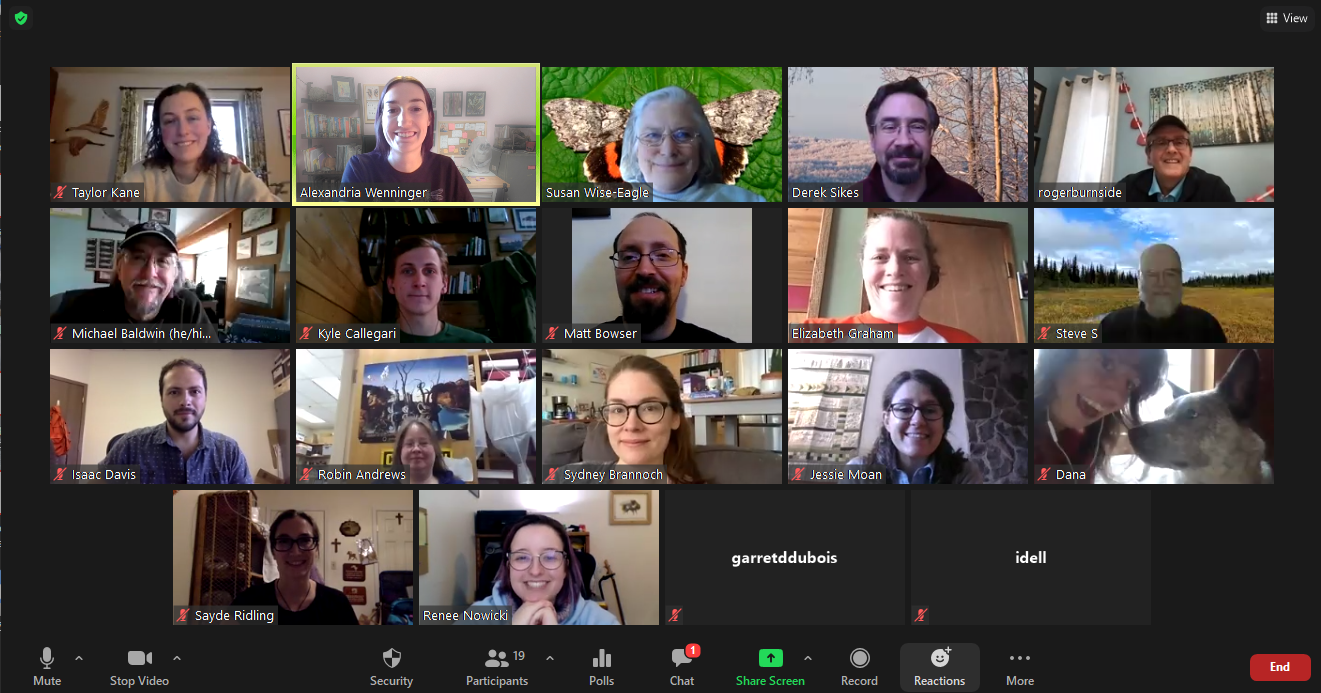
\includegraphics[width=\textwidth]{img/meeting.png}
\caption{Zoom gallery view of the faces of 19 society members that were able to stay for the Society Business Meeting after the 14\textsuperscript{th} annual meeting. From left to right, top row: Taylor Kane, Alex Wenninger, Susan Wise-Eagle, Derek Sikes, Roger Burnside. Second row: Mike Baldwin, Kyle Callegari, Matt Bowser, Liz Graham, Steve Swenson. Third row: Isaac Davis, Robin Andrews, Sydney Brannoch, Jessie Moan, Dana Brennan. Fourth row: Sayde Ridling, Renee Nowicki, Garret Dubois, Isaac Dell. Photo by Alex Wenninger.}
\label{meeting_photo}
\end{center}
\end{figure} 
\begin{multicols}{2} 

Due to the risks posed by the ongoing SARS-CoV-2/Covid-19 pandemic, the Alaska Entomological Society Meeting held its first ever virtual annual meeting via the platform ‘Zoom’ on 30 January 2021. 

\section{Presentations}

In her talk titled ``Hemlock sawfly in Southeast Alaska: using an interdisciplinary approach to monitor a large-scale defoliation event'', \textbf{Liz Graham} walked us through several ways that she and Karen Hutton of the US Forest Service’s Forest Health Protection unit have modified their monitoring protocols during the pandemic. One of their most notable methods was to use high resolution satellite imagery to monitor a hemlock sawfly outbreak. Liz stresses the importance of using multiple methods to monitor insect outbreaks.

\textbf{Todd Sformo} gave an insightful talk about his thesis work which he had conducted in Fairbanks, Alaska on the overwintering physiology of insects, and their strategies for freeze tolerance and avoidance. After, he read aloud a literary piece he originally published in the journal \href{https://catamaranliteraryreader.com/}{\textit{Catamaran}} titled ``So much depends upon\ldots{}'' which gave a heartfelt view of the frustrations and triumphs of studying insects in Alaska. His literary piece can be found in the Fall 2020, Volume 8, Issue 3 publication of the journal \textit{Catamaran}. Todd currently works for the Department of Wildlife Management in the North Slope Borough. 

\textbf{Jessica Rykken} shared insights from her state-wide survey tracking plant phenology and pollinator diversity across Alaskan National Parks in her talk titled ``Flies rule! Exploring the full diversity of arthropod flower-visitors on common Alaskan plants''. Jessica works as an entomologist in Denali National Park and is an expert in pollinators, and through this work sought to not only get a broader understanding of the range of floral-visiting arthropods across eight National Parks in the state, but also to get a baseline for the timing of floral availability and their arthropod visitors to compare to in the future as the climate warms. 

Through his talk titled ``Life history of Alaska’s only Mygalomorph spider'', \textbf{Joey Slowik} gave a fantastic overview of the spider \textit{Antrodiaetus pacificus} including its habits and life cycle, as well as his efforts to survey its distribution in Southeast Alaska. Working with this spider is challenging because they have very isolated populations and they are cryptic in nature. Molecular work done by Joey suggests the Southeast Alaskan island populations of this spider are genetically distinct from the species on the mainland, and additionally due to their rarity and specific needs they may be a species of conservation concern. Joey currently works for the \acr{UAF} Cooperative Extension Service out of Palmer. 

\textbf{Jackson Audley} joined us this year to update us on the ongoing semiochemical work with Spruce Beetle in Alaska. Jackson and his colleague Chris Fettig with the Pacific Southwest Research Station of the \acr{USDA} Forest Service have had ongoing experiments throughout the most recent spruce beetle outbreak to try to find methods that work to deter spruce beetle here in Alaska. His talk titled ``An update on spruce beetle research efforts in Alaska and the Rocky Mountains'' gave an overview of his experiments with deterring spruce beetle attack through use of semiochemicals, how Alaskan and Rocky Mountain populations of spruce beetle compare in their response to the same semiochemicals, and plans for new research avenues to explore.

\textbf{Derek Sikes} presented work he and Logan Mullen conducted in his talk titled, ``Phylogeny and evolution of large body size in the rove beetle genus \textit{Phlaeopterus} Motschulsky, 1853 (Coleoptera: Staphylinidae: Omaliinae: Anthophagini). Derek presents evidence that large body size evolved twice in this genus: this work was accepted for publication and will be available soon. Derek also notes that many of these species are associated with alpine snowfields, so the loss of these snowfields as the climate warms poses a conservation risk for these species; two of the newly described species of \textit{Phlaeopterus} haven’t been collected in the last 36 years despite some effort to do so. Derek Sikes is both a professor and researcher at the University of Alaska Fairbanks as well as the Curator of Insects at the University of Alaska Museum of the North. 

\textbf{Curtis Knight} and \textbf{Ben Diehl} followed with a joint presentation of the \acr{USDA} \acr{TASC} (Technical Assistance for Specialty Crops) program in Alaska. Curtis Knight with the Alaska Department of Natural Resources Division of Agriculture covered the ``\href{http://www.akentsoc.org/doc/Knight_C_and_B_Diehl_2021.pdf}{\acr{TASC} overview: Eliminating pest-related trade barriers for the Alaskan peony industry with focus on thrips}''. \textbf{Ben Diehl}, agricultural researcher with Washington State University Mount Vernon Northwestern Washington Research \& Extension Center, covered the ``\href{http://www.akentsoc.org/doc/Knight_C_and_B_Diehl_2021.pdf}{Alaska \acr{USDA} FAS \acr{TASC}: Morphological studies of thrips associated with peonies}.'' The goals of this project are to establish thrips identification tools, conduct both field and post-harvest trials to determine control options against thrips, and to increase outreach with growers through training and workshops. By reaching these goals, the \acr{TASC} project managers hope to reduce the economic impact of thrips for peony growers. 

We had one student presentation and one student poster shared at the meeting this year. We congratulate \textbf{Taylor Kane} (\acr{UAF}), recipient of the 2021 Student Presentation Award, for her talk, ``\href{http://www.akentsoc.org/doc/Kane_T_2021.pdf}{The diversity and distribution of Alaskan \textit{Boreus}}''. Taylor’s research project will address a current gap in knowledge and we are excited to hear more about her findings in the coming years. Congratulations, Taylor! We also congratulate \textbf{Robin Andrews} (\acr{UAF}), recipient of the 2021 Student Poster Award, for her poster titled, ``Soil microarthropods tell tales that vegetation hides.'' Robin has been working with an understudied and challenging group of organisms and we commend her on her persistence. Congratulations, Robin! We also thank this year’s student presentation award judges: Garret Dubois, Roger Burnside, and Alex Wenninger.

\section{Business items---highlights}

\begin{itemize}

\item	A suggestion was made to consider having the annual meeting occur on a week day next year rather than a Saturday. Next year officers will poll the AKEntoNet ListServe with a few preferred dates to choose from before scheduling the meeting.

\item	When we are able to return to in-person meetings, the society will consider having separate meeting rooms in each Anchorage, Fairbanks, and Juneau that are all then connected via Zoom. This way travel is reduced but there is still the in-person experience in each of the three main locations. 

\item	Election results: Dana Brennan (president), Robin Andrews (vice president), Taylor Kane (secretary), and Roger Burnside (treasurer). 

\end{itemize}

The minutes from our business meeting are available on the website.
